\documentclass[conference]{IEEEtran}
\usepackage[pdftex]{graphicx}
\usepackage{url}

% correct bad hyphenation here
\hyphenation{op-tical net-works semi-conduc-tor}

\begin{document}
\title{Asynchronous Arbitration Primitives\\for New Generation of Circuits and Systems\vspace{-3mm}}
\author{\IEEEauthorblockN{Andrey Mokhov\IEEEauthorrefmark{1}, Danil Sokolov, Victor Khomenko, Alex Yakovlev}
\IEEEauthorblockA{Newcastle University, Newcastle upon Tyne, United Kingdom}
\IEEEauthorblockA{\IEEEauthorrefmark{1}\emph{Corresponding author}: \url{andrey.mokhov@ncl.ac.uk}}}

\maketitle

\begin{abstract}
This paper presents an overview of a family of asynchronous arbitration primitives designed
to increase the resilience and efficiency of the new generation of circuits and systems.
We cover primitives for synchronisation and decision-making with an emphasis on interfacing
analog and digital worlds, sampling of non-persistent signals, and efficient handling of
correlated sensor events.
\end{abstract}

% no keywords

\section{Introduction}

The new generation of circuits and systems is breaking conventional walls between
different timing, voltage and technology domains. Modern `synchronous' and `digital'
systems are emphatically asynchronous-at-large and analog-at-heart: they contain tens
to hundreds of timing and voltage domains, some even thousands~\cite{2017_bohnenstiehl_kilocore}.
Asynchronous arbitration primitives are now used both to orchestrate the communication
between different clock domains~\cite{2017_jiang_noc} and to control the analog-digital
interfaces in on-chip power regulators~\cite{2017_sokolov_a4a}.

% Asynchronous arbitration primitives are key to the
% resilience and efficiency of these systems.

This paper presents an overview of the recently developed asynchronous arbitration
primitives that address the problem of interfacing between hazardous and/or analog
worlds and hazard-free asynchronous circuits in a safe way. We cover synchronisation and
decision-making primitives in Sections~\ref{sec-sync} and~\ref{sec-decision}, respectively.
All of the presented circuit specifications and implementations have beed developed using
the open-source asynchronous design tool \textsc{Workcraft}~\cite{Workcraft_website} and are
publicly available under the MIT license~\cite{Arbitration_primitives_github}.

% Asynchronous arbiters are notoriously difficult to design, therefore it is essential to
% use a formal methods for the specification and verification of the ...
% Below we review the language for the formal specification
% of asynchronous circuits, which is used throughout the paper.

\subsection*{STG specification language}\label{sec-stg}

Signal Transition Graphs~(STGs) are commonly used for the specification,
verification and synthesis of asynchronous circuits. See a comprehensive
background on STGs in~\cite{2002_cortadella_book}.

As a brief introduction, let us examine the STG specification shown in
Fig.~\ref{fig:wait}(left/middle). The STG specifies the behaviour
of a circuit with inputs $\{\textsf{sig}, \textsf{ctrl}\}$
and output \textsf{san}. Rising and falling \emph{signal transitions} are depicted by text
nodes, e.g. \textsf{sig+} corresponds to signal \textsf{sig} switching from~0 to~1.
There are also \emph{dummy transitions}, such as \textsf{e}, which do not correspond to
changes of signal values (think of them as abstract events).
Input, output and dummy transitions are conventionally shown in red, blue and black
colour, respectively.

Directed arcs between nodes express the \emph{precedence} relation
between transitions, e.g. arc $\textsf{san+} \longrightarrow \textsf{ctrl-}$ indicates
that input \textsf{ctrl} goes low only after output \textsf{san} goes high.
An arc can be \emph{marked} with a \emph{token}, shown as a black dot, to specify
the initial state of the circuit: the tokens before transitions \textsf{sig+} and
\textsf{ctrl+} imply the initial state \textsf{sig=ctrl=san=0}.

A transition is \emph{enabled} to occur if it has tokens on each of its incoming
arcs, otherwise it is \emph{disabled}, e.g. \textsf{ctrl+} is enabled and \textsf{san-}
is disabled. When a transition occurs, it \emph{consumes} the tokens on its incoming arcs
are \emph{produces} them on its outgoing arcs, e.g. \textsf{ctrl+} moves the token to arc
$\textsf{ctrl+} \longrightarrow \textsf{e}$. Undirected arcs, called
\emph{read arcs}, are used to \emph{test} the existence of a token in a \emph{place}, shown as
a circle (think of it just as a placeholder for a token), e.g. the read arc
$\textsf{sig1} \frac{~~~~}{~} \textsf{e}$ allows the latter to occur only if the place
is marked, i.e. if \textsf{sig=1}.

A transition is \emph{persistent} if, once enabled, it will occur without becoming
disabled again. Non-persistence in an STG specification
often manifests itself as a \emph{hazard} in the circuit implementation, where a signal
can start switching from~0 to~1 but is stopped midway resulting in a short analog pulse.

% Signal transition loop\\
% Handshake\\

\begin{figure}
\begin{center}
    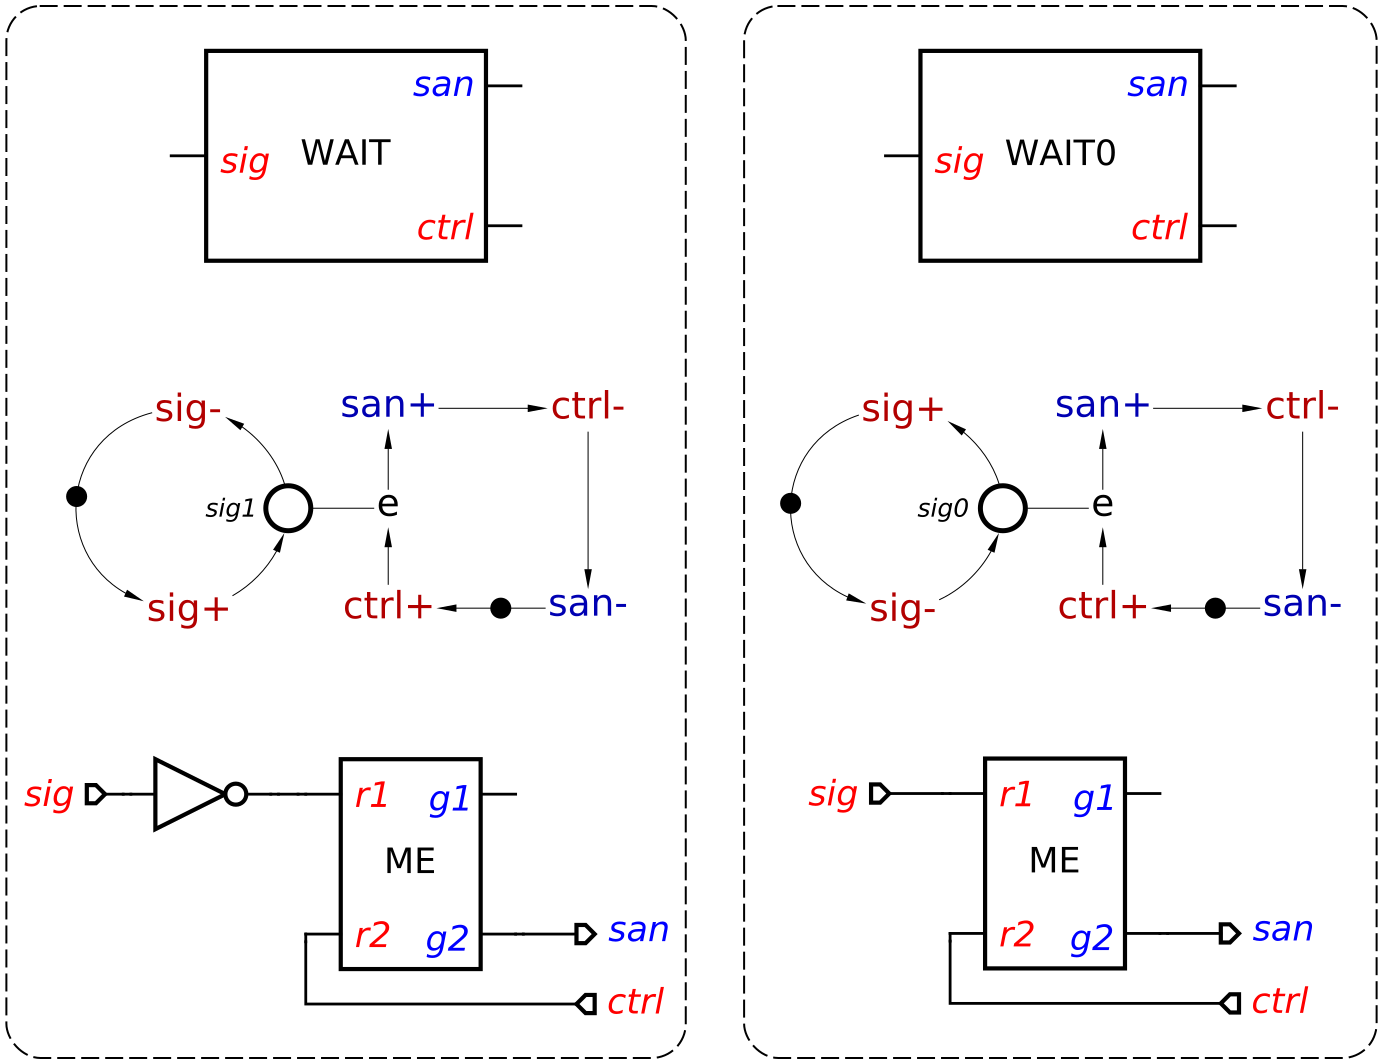
\includegraphics[scale=0.23]{fig/WAIT.pdf}
    \caption{\textsf{WAIT} and \textsf{WAIT0}: block diagram,
    specification and implementation.}
    \label{fig:wait}
    \vspace{-4mm}
\end{center}
\end{figure}

\section{Synchronisation primitives}\label{sec-sync}

This section covers the primitives for the synchronisation of hazard-free signal
transitions in asynchronous circuits with potentially hazardous signals coming
from the environment.
% Note: we use terms `hazard-free' and `persistent' as synonyms.

\subsection{\textsf{WAIT} and \textsf{WAIT0}}

\begin{figure*}
\begin{center}
    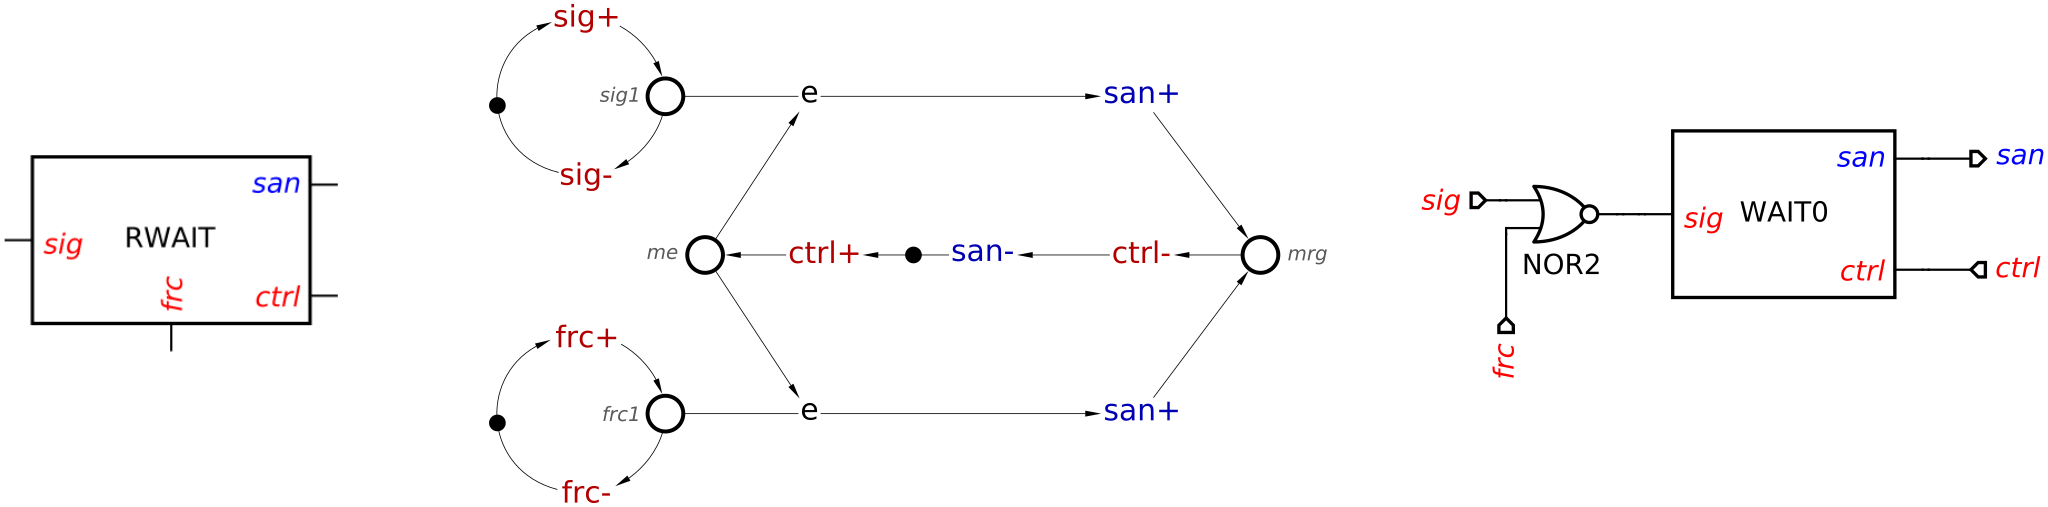
\includegraphics[scale=0.23]{fig/RWAIT.pdf}
    \caption{\textsf{RWAIT}: block diagram, specification and implementation.}
    \label{fig:rwait}
\end{center}
\end{figure*}

The \textsf{WAIT} element~\cite{2015_sokolov_multiphase}, shown in Fig.~\ref{fig:wait}(left),
synchronises the asynchronous handshake \textsf{ctrl/san} with the non-persistent
input~\textsf{sig}. According to the STG specification, \textsf{sig} is unconstrained and
is allowed to switch between~0 and~1 values with no regard to the output handshake -- this
is captured by the loop with signal transitions \textsf{sig+} and \textsf{sig-}.
Initially~\textsf{ctrl=0} and the input is isolated from the output \textsf{san}.
By raising the~\textsf{ctrl} input, the element is switched into the \emph{waiting mode},
where it stays until~\textsf{sig} becomes high. The~\textsf{sig=1} condition enables the dummy
transition~\textsf{e} to fire (via the read arc), thus the output~\textsf{san=1} is produced
and is persistently held\footnote{Here and further on, the output \textsf{san}
is the `sanitised' (persistent) version of the `dirty' (non-persistent) input \textsf{sig}.}
until \textsf{WAIT} is reset by releasing the control input (transition~\textsf{ctrl-}).

Note that an input spike (\textsf{sig+} followed by \textsf{sig-}) in the waiting
mode can be too short fot the \textsf{WAIT} element to register it, in which case it is
ignored. The non-persistent behaviour and the associated metastability is fully contained
within the element, guaranteeing a clean hazard-free output.

The implementation is based on the \emph{mutual-exclusion (ME)
element}~\cite{2008_kinniment_synchronisation}, which is well-known and extensively
studied by the asynchronous circuit design community.

\textsf{WAIT} is a fundamental synchronisation primitive that is used for
implementing other, more sophisticated components presented in this paper.
The symmetric version of the element that waits for the input to become low is
called \textsf{WAIT0}; its top-level block diagram, the STG specification and
the implementation are shown in Fig.~\ref{fig:wait}(right).

\subsection{\textsf{RWAIT} and \textsf{RWAIT0}}

\textsf{RWAIT} and \textsf{RWAIT0} are modifications of the \textsf{WAIT} and \textsf{WAIT0}
elements, respectively, with a possibility to persistently cancel the waiting request. This
is useful when the input is no longer expected to change or the change is no longer relevant
for the asynchronous controller, and hence the output handshake needs to be released.

The top-level diagram of \textsf{RWAIT} is shown in Fig.~\ref{fig:rwait}. The additional input
\textsf{frc} can be used to force the reset of the output handshake in the waiting mode. The
STG specification highlights the fact that the transition \textsf{san+} can be caused either by
\textsf{sig+} or \textsf{frc+}. The implementation reflects the resulting
OR-causality~\cite{1996_yakovlev_or}: inputs \textsf{sig} and \textsf{frc} are simply combined
via a NOR gate, whose output is synchronised with the asynchronous handshake \textsf{ctrl/san}
using the \textsf{WAIT0} element.

The \textsf{RWAIT0} element is implemented analogously.

\subsection{\textsf{WAIT01} and \textsf{WAIT10}}

\textsf{WAIT01} and \textsf{WAIT10} elements wait for a rising or falling edge of the input
signal, respectively. Note, this is subtly different from waiting for high or low input value,
e.g. a signal can be initially low, and to generate a falling edge event it must first go high.

\begin{figure}
\begin{center}
    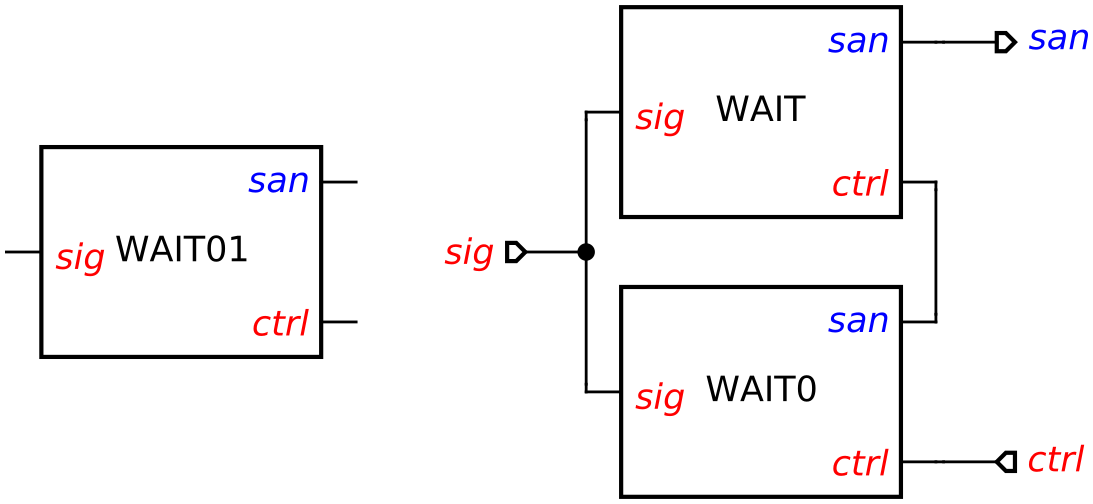
\includegraphics[scale=0.23]{fig/WAIT01.pdf}
    \caption{\textsf{WAIT01}: block diagram and implementation.}
    \label{fig:wait01}
\end{center}
\end{figure}

\subsection{\textsf{WAIT2}}
\textsf{WAIT2} is a combination of \textsf{WAIT} and \textsf{WAIT0} elements:
it uses a 2-phase output handshake, waiting for high and low input values, one after
the other.

\begin{figure}
\begin{center}
    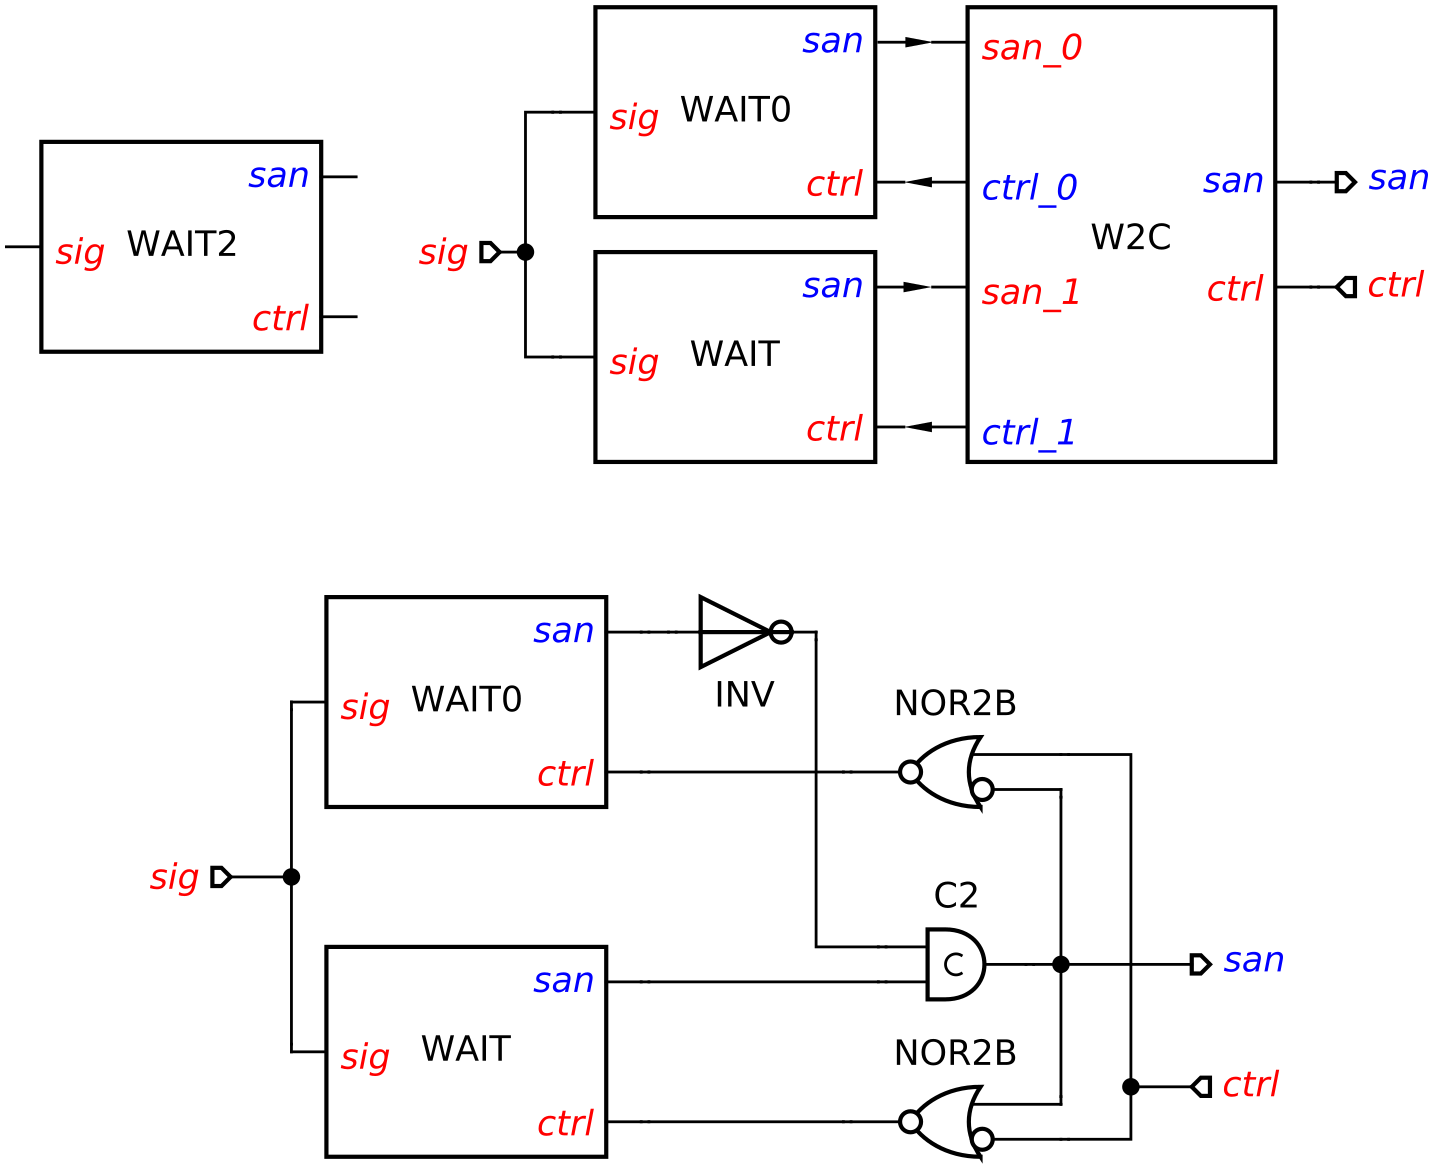
\includegraphics[scale=0.23]{fig/WAIT2.pdf}
    \caption{\textsf{WAIT2}: block diagram and conceptual design (top left and right),
    and implementation (bottom).}
    \label{fig:wait2}
\end{center}
\end{figure}

\section{Decision-making primitives}\label{sec-decision}

This section presents a family of \emph{decision-making} components that perform
non-trivial event arbitration and coordination tasks and rely on the previously
introduced synchronisation primitives.

\subsection{WAITX}
\subsection{WAITX2}
\subsection{SAMPLE}
\subsection{OM}

% \begin{figure}[h!]
% \begin{center}
%   \includegraphics[width=0.84\linewidth]{FIG/ope-chip.pdf}
%   \vspace{-3mm}
%   \caption{Resiliency of asynchronous control under unstable voltage.}
%   \label{fig:voltage-resiliency}
% \end{center}
% \vspace{-7mm}
% \end{figure}

\section{Conclusions}

\section*{Acknowledgements}

\bibliographystyle{unsrt}
\bibliography{publications}

\end{document}
